\documentclass[a4paper, 12pt, twoside]{article}
\usepackage[utf8]{inputenc}
\usepackage[T1]{fontenc}
\usepackage[french]{babel}
\usepackage{lmodern}
\usepackage{ae,aecompl}
\usepackage[top=2.5cm, bottom=2cm, left=3cm, right=2.5cm, headheight=15pt]{geometry}
\usepackage{graphicx}
\usepackage{eso-pic}
\usepackage{array}
\usepackage{url}
\usepackage{hyperref}

% --- IMPORTATION DE LA PAGE DE GARDE ---
\input{pagedegarde}

\title{AI-Sentinel : Système de détection d’intrusions}
\entreprise{Licence MIASHS - Université Paris Nanterre}
\datedebut{26 mars 2026}
\datefin{23 mai 2026}

\membrea{Thirulokkumar Aakkash - 45018080}
\membreb{Cornu Valentin - 45016459}
\membrec{Demian Nicolae - 45014894}

\begin{document}

\pagedegarde

% ==========================================
% REMERCIEMENTS
% ==========================================
\section*{Remerciements}
Nous tenons à remercier l’équipe pédagogique pour ce projet qui nous a permis
d’allier l’intelligence artificielle aux probl´ematiques concr`etes de la cybersécurité.

\newpage
\tableofcontents
\newpage

% ==========================================
% SECTION 1 : INTRODUCTION
% ==========================================
\section{Introduction}
\textbf{AI-Sentinel} est une solution de surveillance con¸cue pour s´ecuriser les infrastructures
critiques. Le syst`eme analyse les m´etadonn´ees de connexion afin d’identifier en temps
r´eel des comportements suspects. L’enjeu est de garantir la disponibilit´e des services
face `a des menaces de plus en plus sophistiqu´ees.

% ==========================================
% SECTION 2 : ENVIRONNEMENT DE TRAVAIL
% ==========================================
\section{Environnement de travail}
Le développement a été réalisé de manière collaborative avec \textbf{GitHub} pour la gestion du code source et \textbf{Overleaf} pour la rédaction de ce rapport. Le système a été testé dans un environnement
\textbf{Linux}, ce qui facilite la manipulation des journaux système.

% ==========================================
% SECTION 3 : DESCRIPTION ET OBJECTIFS
% ==========================================
\section{Description du projet et objectifs}
L’objectif du projet est de fournir une r´eponse rapide face aux cyberattaques. Notre
architecture repose sur une validation stricte des donn´ees ´echang´ees entre les diff´erents
modules.

\begin{figure}[h]
\centering
\IfFileExists{Tux.png}{%
    \includegraphics[width=0.3\textwidth]{Tux.png}%
}{%
    \fbox{\parbox{0.3\textwidth}{\centering Image Tux.png de test Linux}}%
}
\caption{Tux, le pingouin (environnement de test Linux)}
\label{Tux}
\end{figure}

Le tableau \ref{menaces} présente les types d’anomalies que nous avons choisi de traiter.

\begin{table}[h]
\begin{center}
\begin{tabular}{|l|c|l|}
\hline
Type d'anomalie de trafic & Niveau de criticité & Responsable du module \\
\hline
Injection / Paquet corrompu (C) & Élevé & Nicolae \\
\hline
Déviance comportementale (Python) & Moyen & Valentin \\
\hline
Violation d'intégrité de flux & Critique & Aakkash \\
\hline
\end{tabular}
\end{center}
\caption{Types de détections et gestion multi-niveaux du système}
\label{menaces}
\end{table}

\subsection{Analyse de flux en temps réel}
Le système doit être capable de traiter des flux de données continus[cite: 28]. Le module en C assure un filtrage initial pour ne transmettre que les données formatées correctement[cite: 29].

\subsection{Fiabilité et intégrité}
L'objectif secondaire est d'empêcher toute corruption du moteur d'IA. Si le flux de données est interrompu ou modifié, le système doit se mettre en sécurité[cite: 31].

% ==========================================
% SECTION 4 : TECHNOLOGIES
% ==========================================
\section{Bibliothèques, outils et technologies}
Nous avons utilisé le compilateur \textbf{GCC} pour optimiser les performances du module en C. Pour la partie Python, nous avons exploité des bibliothèques de calcul statistique pour analyser les écarts volumétriques et de fréquences du trafic. Les outils d'IA générative ont été intégrés comme assistants de programmation pour valider l'allocation mémoire en C et structurer le pipeline de données.

% ==========================================
% SECTION 5 : TRAVAIL RÉALISÉ
% ==========================================
\section{Travail réalisé}
\begin{itemize}
    \item \textbf{Réalisé} : Module d'interception et d'écriture de fichier de trafic CSV en C, intégration de filtres de couleurs dans le terminal Python pour distinguer visuellement les risques (faible, moyen, critique), algorithme IA d'analyse comportementale et script de contrôle d'intégrité du flux.
    \item \textbf{Non réalisé} : La coupure automatique de l'interface réseau (prévention active) n'a pas pu être intégrée, faute de droits administrateurs étendus sur notre environnement de test.
    \item \textbf{Répartition} : Nicolae s'est chargé du module de capture en C (performance) et il s'est occupé du fichier sentinel\_main.py qui permet de lancer et d'arrêter simultanément, via une interface graphique simple, le module de capture de trafic en C et le moteur d'analyse comportementale en Python, Valentin du moteur d'IA en Python (analyse), et Aakkash de la coordination globale, de l'intégration du pipeline et de la sécurité du flux de confiance.
\end{itemize}

% ==========================================
% SECTION 6 : DIFFICULTÉS
% ==========================================
\section{Difficultés rencontrées}
La principale difficulté a été  d’assurer une communication fiable entre le module en
C et le programme Python. Il a fallu définir un format de données clair afin d’éviter
les erreurs lors du traitement des fichiers CSV. Nous avons aussi dû gérer les lignes
incomplètes, les caractères inattendus et les journaux suspects. Les tests ont demandé
du temps, car plusieurs cas devaient être simulés pour vérifier la fiabilité du système.
Ces difficultés nous ont permis de mieux comprendre l’importance d’une architecture
simple, robuste et sécurisée.

% ==========================================
% SECTION 7 : BILAN
% ==========================================
\section{Bilan}
\subsection{Conclusion}
Le projet atteint ses objectifs en proposant un système capable d’analyser des journaux et de repérer des anomalies. L’utilisation du C permet un filtrage rapide, tandis
que Python facilite l’analyse et la détection intelligente. Cette organisation rend le projet plus clair, plus fiable et plus simple à faire évoluer. Même si certaines améliorations restent possibles, comme l’ajout d’alertes automatiques, la base du système est fonctionnelle. Ce travail nous a permis de mettre en pratique nos compétences en programmation et en cybersécurité.

\subsection{Perspectives}
Une amélioration possible serait l’ajout d’une interface graphique pour visualiser
les alertes en temps r´eel sur un tableau de bord.

\newpage

% ==========================================
% BIBLIOGRAPHIE ET WEBOGRAPHIE
% ==========================================
\section{Bibliographie}
\begin{thebibliography}{1}
   \bibitem[LAM94]{lam1} L. Lamport, {\it \LaTeX{}: A Document Preparation System}, Addison-Wesley, 1994.
\end{thebibliography}

\newpage

\section{Webographie}
\begin{thebibliography}{1}
   \bibitem[GH]{gh} Dépôt public du projet : \url{https://github.com/aakkashthirulo-spec/AI-Sentinel}
\end{thebibliography}

\newpage

% ==========================================
% ANNEXES
% ==========================================
\appendix
\makeatletter
\def\@seccntformat#1{Annexe~\csname the#1\endcsname:\quad}
\makeatother

\section{Cahier des charges}
Le système doit auditer en continu le trafic réseau afin d'isoler les comportements malveillants. Le programme en C réalise un contrôle de formatage amont, puis le script Python interprète les résultats statistiques. En cas de flux corrompu ou d'altération du fichier intermédiaire, le programme doit immédiatement lever une alerte critique et se mettre en sécurité.

\section{Exemple d'exécution du projet}
\begin{figure}[h]
\centering
\IfFileExists{capture_sentinel.c.png}{%
    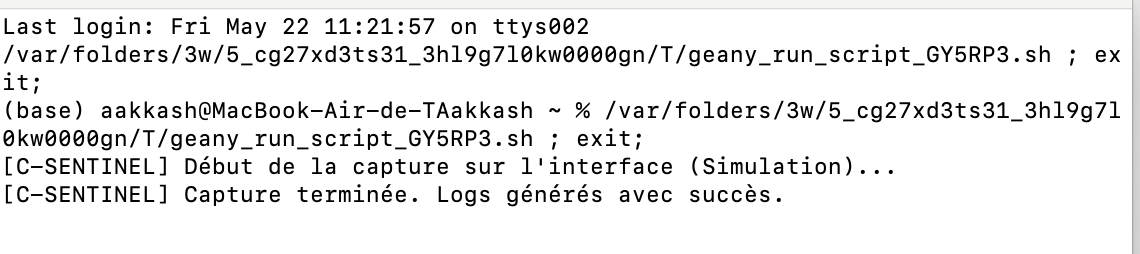
\includegraphics[width=0.8\textwidth]{capture_sentinel.c.png}%
}{%
    \fbox{\parbox{0.8\textwidth}{\centering \vspace{1.5cm} [Capture d'écran 1 : Exécution du module C de capture réseau] 
    \vspace{1.5cm}}}%
}
\caption{Capture d'écran du terminal lors de la capture des flux par le module C.}
\end{figure}

\begin{figure}[h]
\centering
\IfFileExists{capture_sentinel.py.png}{%
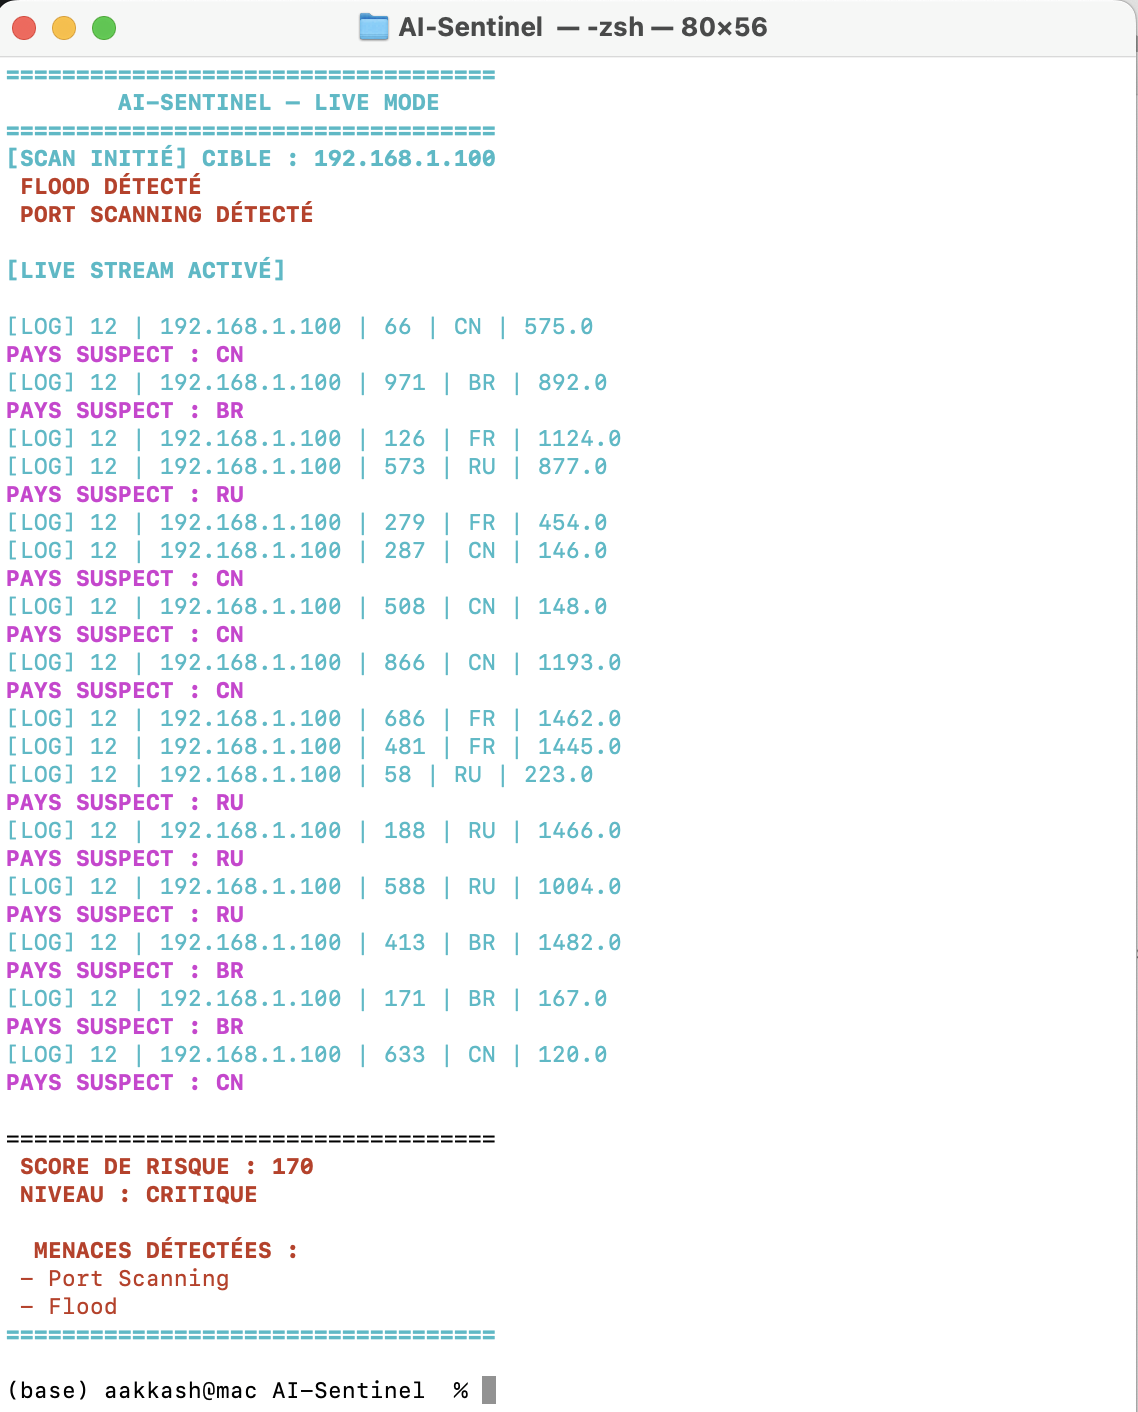
\includegraphics[width=0.8\textwidth,height=0.35\textheight,keepaspectratio]{capture_sentinel.py.png}%
}{%
    \fbox{\parbox{0.8\textwidth}{\centering \vspace{1.5cm} [Capture d'écran 2 : Alerte Python d'anomalie comportementale] \vspace{1.5cm}}}%
}
\caption{Détection d'une anomalie volumétrique par le moteur IA en Python.}
\end{figure}

\section{Manuel utilisateur}
Pour exécuter le système complet de surveillance, ouvrez votre terminal Linux et lancez la commande suivante :
\begin{verbatim}
python3 sentinel_main.py trafic_reseau.csv
\end{verbatim}

\end{document}